\documentclass[12pt,a4paper]{article}
\usepackage{amsmath,graphicx}
\title{Normal distribution}
\author{Wikipedia, the free encyclopedia}
\date{April 18, 2019}

\begin{document}
\maketitle
\section{Introduction}
In probability theory, the normal distribution is a very common continuous probability
distribution. Normal distributions are important in statistics and are often used in the natural
and social sciences to represent real-valued random variables whose distributions are not known.
A random variable with a Gaussian distribution is said to be normally distributed and is called a
normal deviate.

\begin{figure}[h]
  \centering
  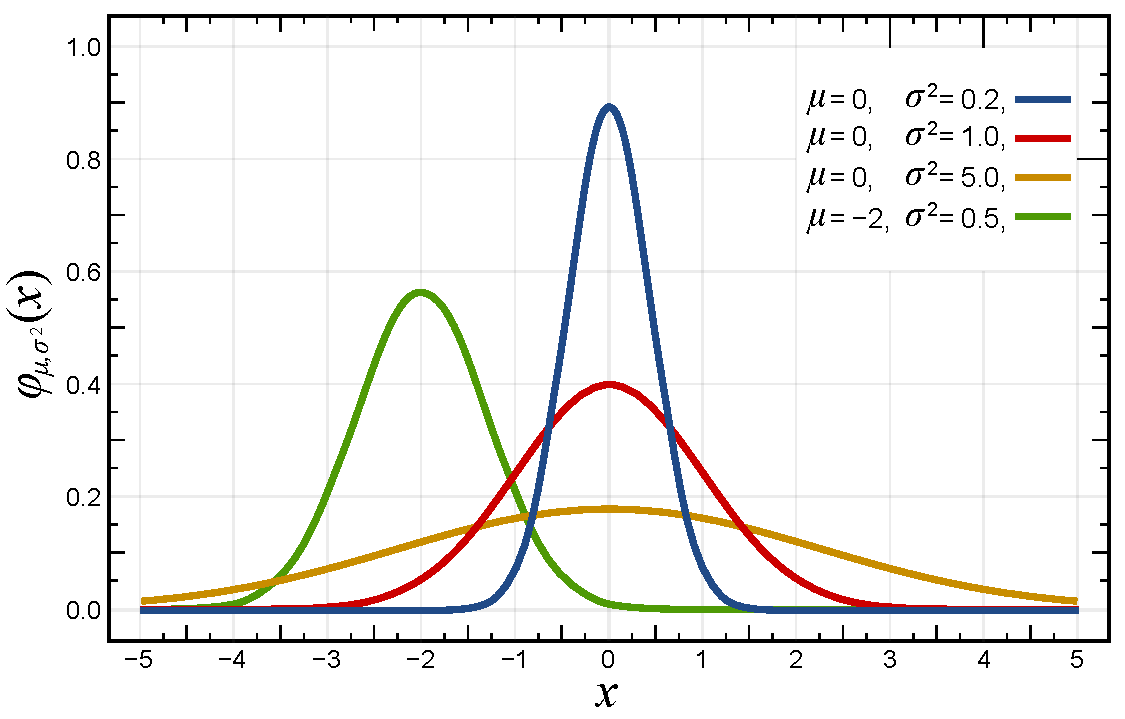
\includegraphics[width=8cm]{normal-distribution-PDF.pdf}
\end{figure}

The probability density of the normal distribution is
\begin{equation}
  f(x|\mu,\sigma)
  = \frac{1}{\sqrt{2\pi\sigma^2}}
    e^{-\frac{(x-\mu)^2}{2\sigma^2}}
\end{equation}
where
\begin{itemize}
  \item $\mu$ is the mean of the distribution
  \item $\sigma$ is the standard deviation
\end{itemize}
\end{document}
